\documentclass[a4paper,titlepage,onecolumn]{report}
\usepackage{amsmath}
\usepackage{graphicx} % required for pdf transparency
\usepackage{xcolor} % required for pdf transparency
\usepackage{amsthm}
\usepackage{amssymb}
\usepackage{booktabs}
\usepackage{tabularx}
\usepackage{subfigure}
\usepackage{mathrsfs}
\usepackage{textcomp}
\usepackage{siunitx}
\usepackage{fullpage}
\usepackage[multiple]{footmisc}
\usepackage{hyperref}
\usepackage{multirow}
\usepackage{empheq}
\usepackage{calc}
\usepackage[version=3]{mhchem}
\usepackage{tikz}
\usepackage{pgfplots}
\usepackage{xcolor}
\usepackage[section]{placeins}
\pgfplotsset{compat=newest}


%\hypersetup{
% colorlinks=false,
% linkbordercolor={1 1 1},
% citebordercolor={1 1 1},
% urlbordercolor={1 1 1} 
%}

\sisetup{ 
% load-configurations=abbreviations
% round-mode = places,
}%

% New definition of square root:
% it renames \sqrt as \oldsqrt
% This definition puts a little vertical guy at the end so it's more
% obvious where the square root actually ends.
\let\oldsqrt\sqrt
% it defines the new \sqrt in terms of the old one
\def\sqrt{\mathpalette\DHLhksqrt}
\def\DHLhksqrt#1#2{%
\setbox0=\hbox{$#1\oldsqrt{#2\,}$}\dimen0=\ht0
\advance\dimen0-0.2\ht0
\setbox2=\hbox{\vrule height\ht0 depth -\dimen0}%
{\box0\lower0.4pt\box2}}

% integrals with infinity bounds
\newcommand{\intinfty}{\int_{-\infty}^{\infty}}

% consistent formatting of object labels
\newcommand{\Figure}[1]{Figure \ref{#1}}
\newcommand{\Equation}[1]{Equation \ref{#1}}
\newcommand{\Table}[1]{Table \ref{#1}}
\newcommand{\Section}[1]{Section \ref{#1}}
\newcommand{\Chapter}[1]{Chapter \ref{#1}}
\newcommand{\Appendix}[1]{Appendix \ref{#1}}

% missing mathematical operators
\DeclareMathOperator{\sinc}{sinc}
\DeclareMathOperator{\sech}{sech}
\DeclareMathOperator{\sgn}{sgn}
\DeclareMathOperator{\erf}{erf}
\DeclareMathOperator{\inverf}{inverf}
\DeclareMathOperator{\arcsinh}{arcsinh}
\DeclareMathOperator{\arccosh}{arccosh}
\DeclareMathOperator{\arctanh}{arctanh}
%\DeclareMathOperator{\Re}{Re}
%\DeclareMathOperator{\Im}{Im}

% use roman type for natural base e and sqrt(-1)
\newcommand{\me}{{\mathrm{e}}}
\newcommand{\mi}{{\mathrm{i}}}

% roman type for the derivative, plus a space
\newcommand{\md}{\,\mathrm{d}}

% fourier transform and the reverse
\newcommand{\ff}[1]{{\mathscr{F}^{+}\bigl(#1\bigr)}}
\newcommand{\fr}[1]{{\mathscr{F}^{-}\bigl(#1\bigr)}}

% hilbert transform and the reverse
\newcommand{\hf}[1]{{\mathscr{H}^{+}\bigl(#1\bigr)}}
\newcommand{\hr}[1]{{\mathscr{H}^{-}\bigl(#1\bigr)}}

% custom lengths for figures

% width for side by side figures
\newlength{\twoupwidth}
\setlength{\twoupwidth}{7.5cm}

% width and height for default single figure
\newlength{\oneupwidth}
\setlength{\oneupwidth}{0.90\textwidth}
\newlength{\oneupheight}
\setlength{\oneupheight}{0.55623059\textwidth}

% custom colors for 2D plots - these are the same ones mathematica uses by
% default
\definecolor{colora}{RGB}{63,61,153}
\definecolor{colorb}{RGB}{153,61,113}
\definecolor{colorc}{RGB}{153,139,61}
\definecolor{colord}{RGB}{61,153,86}
\definecolor{colore}{RGB}{61,90,153}
\definecolor{colorf}{RGB}{153,61,144}
\definecolor{colorg}{RGB}{153,109,61}
\definecolor{colorh}{RGB}{67,153,61}
\definecolor{colori}{RGB}{61,121,153}
\definecolor{colorj}{RGB}{132,61,153}

% hilight text... a "work in progress" type thing
\tikzstyle{todobox} = [draw=red, fill=blue!10, very thick,
rectangle, rounded corners, inner sep=10pt, inner ysep=20pt]
\tikzstyle{todotitle} =[fill=red, text=white]

\newcommand{\todo}[1]{%
\begin{center}
\begin{tikzpicture}
\node [todobox] (box){%
 \begin{minipage}{0.9\textwidth}
 #1
 \end{minipage}
};
\node[todotitle, right=10pt] at (box.north west) {To Do:};
\end{tikzpicture}
\end{center}

}

\pgfplotsset{
 /pgfplots/colormap={jet}{rgb255(0cm)=(0,0,128) rgb255(1cm)=(0,0,255)
 rgb255(3cm)=(0,255,255) rgb255(5cm)=(255,255,0) rgb255(7cm)=(255,0,0)
 rgb255(8cm)=(128,0,0)}
}
\usepgfplotslibrary{units}
\usetikzlibrary{pgfplots.units} 


\pdfpageattr {/Group << /S /Transparency /I true /CS /DeviceRGB>>} 

\begin{document}

%%%%% TITLE PAGE %%%%%
\begin{titlepage}
\begin{center}
\hfill\\[4cm]
{ \Huge {\bfseries {Interference and Scattering in Surface Plasmon Resonance}} \par}
\vspace{3.0cm}
\begin{tabular}{lr}

\includegraphics[height=2cm,keepaspectratio]{logo/Logo_MPL_englisch_kompakt_cmyk_110915}
\hspace{1.0cm}
%
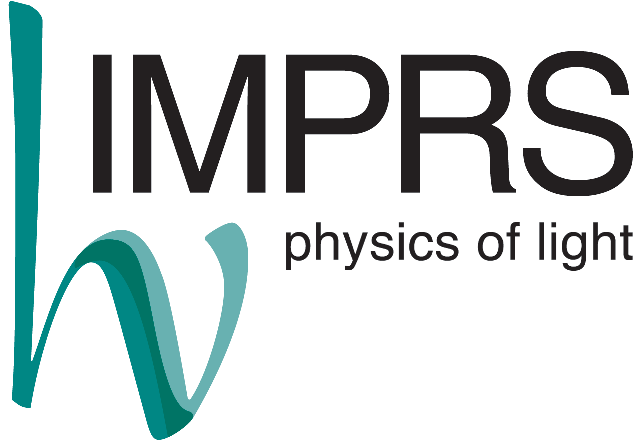
\includegraphics[height=2cm,keepaspectratio]{logo/Logo_IMPRS_4c_042012}
\end{tabular}
\vspace{3cm}
\\
{\huge Aaron Webster}\\
\vspace{1cm}
{\large A DISSERTATION}\\
\vspace{0.5cm}
Presented to the Max Planck Institute for the Science of Light\\
and the University of Erlangen-N\"urnberg\\
in partial fulfillment of the requirements\\
for the degree of\\
Doctor of Philosophy\\
\vspace{0.5cm}
\today
\end{center}
\end{titlepage}

%%%%% DECLARATION OF ORIGINALITY %%%%%
\chapter*{Declaration of Originality}
I affirm that the work presented in this dissertation is, to the best of my
knowledge, original and my own, except as acknowledged in the
text. \\
\hfill\\[1cm]
Signed\hspace{0.25cm}\makebox[5cm]{\hrulefill}\hspace{0.25cm}(Aaron Webster)
\hfill\\[1cm]
Date\hspace{0.51cm}\makebox[5cm]{\hrulefill}\hspace{0.25cm}
\vspace{2cm}

%%%%% ADVISOR, CO-ADVISOR %%%%%
\section*{Evaluation Committee}
\subsection*{First Advisor}
Dr. Frank Vollmer\\
Laboratory of Biophotonics and Biosensing\\
Max Planck Institute for the Science of Light\\
G\"unther-Scharowsky-Str.1 / Bau 24\\
91058 Erlangen
\subsection*{Second Advisor}
Prof. Dr. Ulf Peschel\\
Institute of Optics, Information and Photonics\\
University Erlangen-N\"urnberg\\
G\"unther-Scharowsky-Str.1 / Bau 24\\
91058 Erlangen

\newpage
%%%% ACKNOWLEDGEMENTS %%%%
\chapter*{Acknowledgements}
I would like to extend my gratitude to the following individuals who helped
me throughout this work: to Jiapeng Huang, for his enthusiasm and hard work
in carrying out many tedious but necessary experiments, to Dr. Yuqiang Wu
for determining out the proper protocols regarding the use of DNA origami,
to Dr. Matthew Foreman for many insightful theoretical endevours, and to
Professor Stephen Gregory and Dr. R.P. Schumann whose pioneering work
inspired this dissertation.

%%%%% TABLE OF CONTENTS &&&&&
\pagenumbering{roman}
\tableofcontents

%%%%% ABSTRACT %%%%%
\begin{abstract}
(abstract is written last)
\end{abstract}
% the first part is in roman numbering, switch now to arabic
\pagenumbering{arabic}

\chapter{Foundations}
\section{Synopsis}
This dissertation is all about what happens when surface plasmons are
scattered in a prism coupled setup.  The easiest way of understanding this
is though the experimental setup, shown below in \Figure{fig:kretschmanngeo}.  
\begin{figure}[hb]
\centering
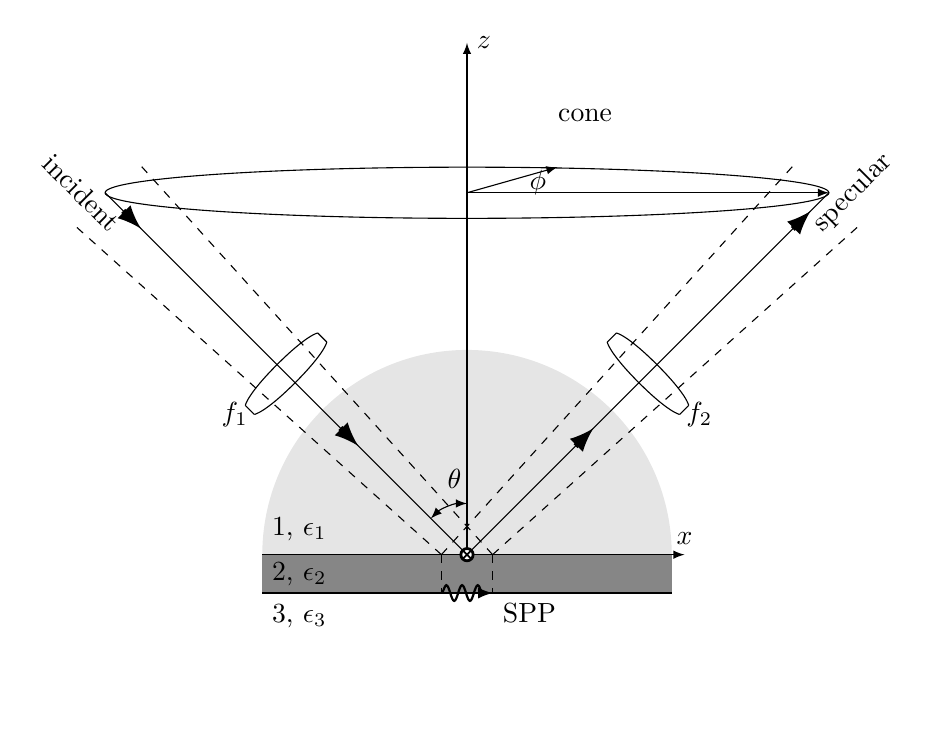
\begin{tikzpicture}[
    scale=0.65,
    >=latex,
    media/.style={font={}},
    wave/.style={
        decorate,decoration={snake,post length=1.0mm,amplitude=1mm,
        segment length=2.0mm},thick},
    interface/.style={
        % The border decoration is a path replacing decorator.
        % For the interface style we want to draw the original path.
        % The postaction option is therefore used to ensure that the
        % border decoration is drawn *after* the original path.
        postaction={draw,decorate,decoration={border,angle=-45,
                    amplitude=0.3cm,segment length=2mm}}},
    ]

    \def\thetasp{45}
    \def\spread{10}
    \def\wx{1}
    \def\conedist{10}

    % glass
    \fill[gray!20] (4,0) arc (0:180:4);

    % air
    \fill[gray!0] (-4,-3) rectangle (4,0);

    % metal
    \fill[gray!95] (-4,-0.75) rectangle (4,0);

    % Interface
    \draw[black,line width=.5pt](-4,0)--(4,0);
    \draw[black,line width=.5pt](-4,-0.75)--(4,-0.75);

    % Vertical dashed line
    %\draw[dashed,gray](0,-3)--(0,3);
    % Coordinates system
    \draw[<->] (4.25,0) node[above]{$x$}-|(0,10) node[right]{$z$};
    \draw[->] (0,{cos(\thetasp)*\conedist}) -- ({sin(\thetasp)*\conedist}, {cos(\thetasp)*\conedist});
    \draw[->] (0,{cos(\thetasp)*\conedist}) --
    ({0.25*cos(\thetasp)*\conedist}, {0.5+sin(\thetasp)*\conedist})
    node[shift={(-0.25,-0.20)}] {$\phi$} ;

    \node[shift={(1.5,{sin(\thetasp)*\conedist-1.5})}] {cone};

    % cone
    \draw (0,{cos(\thetasp)*\conedist}) ellipse ({sin(\thetasp)*\conedist} and 0.5);

    % Incidence
    %\draw[->,wave]
    %     (135:3.2cm)--(135:2.5cm)node[right]{$E_0$};
    \draw[dashed](0:{\wx*-0.5})--({90+\thetasp+\spread*0.5}:10);
    \draw[](0:0)--({90+\thetasp}:10) node[rotate={270+\thetasp}, shift={({0.30*cos(270-\thetasp)},{0.30*sin(270-\thetasp})}] {incident};
    \draw[<->] (0,1) arc (90:{90+\thetasp}:1) node[shift={(0.3,0.5)}] {$\theta$};
    \draw[->,line width=2pt]({90+\thetasp}:9.5)--({90+\thetasp}:9.0);
    \draw[->,line width=2pt]({90+\thetasp}:3.5)--({90+\thetasp}:3.0);
    \draw[dashed](0:{\wx*0.5})--({90+\thetasp-\spread*0.5}:10);
    %\draw[->](0,0.75)arc(90:135:.75cm);

    % Reflection
    %\draw[->,wave]
    %     (45:2.5cm)--(45:3.2cm)node[right]{$E_r$};
    \draw[dashed](0:{\wx*-0.5})--({90-\thetasp+\spread*0.5}:10);
    \draw[](0:0)--({90-\thetasp}:10) node[rotate={90-\thetasp},
    shift={({0.30*cos(270+\thetasp)},{0.30*sin(270+\thetasp})}] {specular};
    \draw[<-,line width=2pt]({90-\thetasp}:9.5)--({90-\thetasp}:9.0);
    \draw[<-,line width=2pt]({90-\thetasp}:3.5)--({90-\thetasp}:3.0);
    \draw[dashed](0:{\wx*0.5})--({90-\thetasp-\spread*0.5}:10);
    \draw[dashed]({\wx*0.5},0)--({\wx*0.5},-0.75);
    \draw[dashed]({-\wx*0.5},0)--({-\wx*0.5},-0.75);
    \draw[->,wave,color=black]
     ({-\wx*0.5},-0.75)--({\wx*0.5},-0.75) node[right,shift={(0,-0.25)}]{SPP};


    % first lens
    \def\lenswidth{2}
    \def\lensheight{0.25}
    \def\lensbow{0.125}
    \def\lensshift{({-5*sin(\thetasp)},{5*cos(\thetasp)})}
    \def\lensrotate{\thetasp}
    \draw[shift={\lensshift}, rotate={\lensrotate}]({-\lenswidth/2},{-\lensheight/2})--({-\lenswidth/2},{\lensheight/2});
    \draw[shift={\lensshift}, rotate={\lensrotate}]({\lenswidth/2},{-\lensheight/2})--({\lenswidth/2},{\lensheight/2});
 
    \draw[shift={\lensshift}, rotate={\lensrotate}] plot [smooth, tension=1.5] coordinates {
    ({\lenswidth/2},{-\lensheight/2})
    (0,{-\lensheight/2-\lensbow})
    ({-\lenswidth/2},{-\lensheight/2})
    } node[shift={(-0.25,0)}] {$f_1$};

    \draw[shift={\lensshift},rotate={\lensrotate}] plot [smooth, tension=1.5] coordinates {
    ({-\lenswidth/2},{\lensheight/2})
    (0,{\lensheight/2+\lensbow})
    ({\lenswidth/2},{\lensheight/2}) };
 
    % second lens
    \def\lensshift{({5*sin(\thetasp)},{5*cos(\thetasp)})}
    \def\lensrotate{-\thetasp}
    \draw[shift={\lensshift}, rotate={\lensrotate}]({-\lenswidth/2},{-\lensheight/2})--({-\lenswidth/2},{\lensheight/2});
    \draw[shift={\lensshift}, rotate={\lensrotate}]({\lenswidth/2},{-\lensheight/2})--({\lenswidth/2},{\lensheight/2});
 
    \draw[shift={\lensshift}, rotate={\lensrotate}] plot [smooth, tension=1.5] coordinates {
    ({-\lenswidth/2},{-\lensheight/2})
    (0,{-\lensheight/2-\lensbow})
    ({\lenswidth/2},{-\lensheight/2})
    } node[shift={(0.25,0)}] {$f_2$};

    \draw[shift={\lensshift},rotate={\lensrotate}] plot [smooth, tension=1.5] coordinates {
    ({-\lenswidth/2},{\lensheight/2})
    (0,{\lensheight/2+\lensbow})
    ({\lenswidth/2},{\lensheight/2}) };


   % Media names
    \path[media] (-4,.5)  node[anchor=west] {1, $\epsilon_1$}
                 (-4,-.375) node[anchor=west] {2, $\epsilon_2$}
                 (-4,-1.2) node[anchor=west] {3, $\epsilon_3$};

    % $x$ axis
    \filldraw[fill=white,line width=1pt](0,0)circle(.12cm);
    \draw[line width=.6pt] (0,0)
                          +(-135:.12cm) -- +(45:.12cm)
                          +(-45:.12cm) -- +(135:.12cm);
    % To-paths are really useful for drawing curved lines. The above
    % to path is equal to:
    %
    % \draw[-latex,thick](3.2,0.5)node[right]{$\mathsf{S_{1,2}}$}
    %      ..controls +(180:.2cm) and +(up:0.25cm) .. (3,0);
    % Internally the to path is translated to a similar bezier curve,
    % but the to path syntax hides the complexity from the user.

    % SPP
    %\draw[->,wave,color=black]
    %     (-2,-1.75)--(2,-1.75) node[right]{SPP};

\end{tikzpicture}

\vspace{-1cm}
\caption{
Experimental setup.
} 
\label{fig:kretschmanngeo} 
\end{figure}
The setup consists of a dielectric hemisphere, upon whose
hypotenuse is deposited a thin layer (\SI{50}{\nano\meter}) of metal.
Light is incident from the left and focussed by a lens
$f_1$ on to the hypotenuse of a hemispherical prism coated with a thin
layer of silver.  

The evanescent wave present on the $\epsilon_1$-$\epsilon_2$ boundary with
a wavenumber $k_x = k_0\sqrt{\epsilon_1}\sin \theta$ has an angle such that
it excites surface plasmon polaritions (SPPs).  SPPs are essentially
oscillations of free charge in the $\epsilon_2$ layer which are coupled to
the photons of the incident beam (polaritions are quasiparticles, but are
still quantum-mechanical in nature).  The majority of light is directed
into the specular direction, while surface roughness causes re-radiation of
the plasmon field into a hollow cone.  $f_2$ acts to image light exiting
the system.

In the specular direction, the re-radiation of SPPs as photons at their
excitation angle will be antiphase with the excitation beam.  The result is
an interference, a dark band in the reflection about a certain range of
angles.  SPPs will propagate on the $\epsilon_2$-$\epsilon_3$ layer until
they either decay as heat or scatter into the far field.  During this
propagation it is possible that surface roughness will elastically modify
its $k$-vector in the $k_x$-$k_y$ plane.  When this happens, scattered SPPs
will re-radiate into a thin annular cone at (nearly) the same angle as the
dark band in the specular direction.

The conically scattered light is what we're interested in.  This light
contains a wealth of information related to SPP scattering.  Most
importantly, this light contains speckle, a seemingly random interference
pattern resulting from many components with different phase relationships.

\section{What is New Here}
In many large works it is sometimes difficult to discern what is actually
new from rehashings of things others have done.  This section is intended
to clarify this situation.  To this accord, the following is a list of new
results presented here
\begin{description}
\item[Interference of Scattered SPPs]
For SPPs excited in the Kretschmann configuration with a focussed beam
whose propagation distance is larger than focal spot, a one-sided
interference pattern is observed in the specular direction.  This was
thought to be an interference effect between the specularly reflected beam
and a re-radiated plasmon component.  We have discovered that that this is
simply a consequence of causality and the interference pattern may be
observed in conically scattered light from the same system.
\item[Sensitivity of Wiggles] 
Using Fourier analysis, we have studied the sensitivity of SPR in an intensity
interrogation configuration as a function of propagation distance.  This
provides a useful measure of the sensitivity of the one-sided interference
pattern found in the specular and conically directed beams.
\item[Refractive Index Sensing With Conical Speckle]
If the surface is rough, the conically directed light contains speckle.  We
have analyzed the speckle patterns as a function of changes in bulk
refractive index.
\item[SPP Nanoparticle Scattering]
Using the speckle in the cone, we observe the changes in intensity and
correlation functions associated with the addition or motion of a single
nanoparticle.
\end{description}

\section{Historical Perspective}
The theoretical groundwork for the existence of surface plasmon polaritons
(SPPs) was first introduced by Richie in his seminal 1957 paper
\textit{Plasma Losses by Fast Electrons in Thin Films}
\cite{ritchie1957plasma}.  Like any scientific work, Richie's was
incremental and has its roots in earlier theoretical proposals by Pines and
Bohm~\cite{bohm1951collective}~\cite{pines1952collective}.  Ultimately this
research functioned to explain the phenomena of sharp and spectrally narrow
energy losses observed in diffraction gratings by Wood in 1902, known as
``Wood's anomaly''.

Optical excitation of surface plasmons was made accessible through
pioneering work in the late 1960's by Kretschmann~\cite{kretschmann1968},
Raether~\cite{raether1965springer} and Otto~\cite{otto1968excitation}.
These experiments used the principle of attenuated total reflection (ATR)
to excite surface plasmons evanescently, using a prism to match their
resonance condition.  A great deal of understanding on the topic of surface
plasmons took place in the subsequent decade, such as an improved
theoretical understanding based on Fresnel relations
\cite{chen1976excitation} and descriptions of of conically scattered light
in the presence of surface roughness~\cite{simon1976directional}.  A
concise overview of this research can be found in~\cite{raether1997surface}.

The introduction of SPR as a biosensing platform began in the early 1980's
with work by Liedberg, Nylander and Lundstrom~\cite{liedberg1983surface}
who described the extraordinary sensitivity of the surface plasmon
resonance condition to perturbations in the refractive index of the medium
on one side of the film.  The subsequent commercialization of SPR
biosensors has largely been influenced by these authors and Pharmacia
Biosensor AB (now Biacore)~\cite{liedberg1995biosensing}.

The commercial success of biosensors based on surface plasmon resonance
seems to have brought about a knowledge gap between the biosensing
community and their more theoretical predecessors from whom the field owes
its genesis.  This is to say that the scope of SPR biosensing experiments
is disproportionately narrower than the breadth of phenomena discovered
since Richie.  As an example particular to this dissertation, in 2005 and
2007, two papers~\cite{andaloro2005optical}~\cite{simon2007observation}
based on theoretical work by Chuang~\cite{chuang1986lateral} and Chen
\cite{chen1976excitation} reported a curious interference pattern occurring
in the specularly reflected light for certain (among them,
Kretschmann-Raether type) systems illuminated with focused Gaussian beams.
This was also independently reported a year later in
\cite{schumann2008near}.  Interestingly, observation of this interference
required nothing more than the addition of a lens pair to a fairly
ubiquitous optical setup, but it somehow escaped attention during earlier
research.  

Many of the topics here are inspired by work done at the University of
Oregon in the labratory of Prof\@.~Stephen Gregory, summarized in a 2009
thesis \textit{Surface Plasmon Random Scattering and Related Phenomena}
\cite{schumann2009surface} by Dr\@.R\@.P\@.~Schumann.  Here is described
experiments performed on thin metal films in a Kretschmann-Raether
configuration with the addition of a scanning apertureless near-field
probe.  This probe (a sharp tungsten tip) is able to elastically scatter
SPPs in a way analogous to surface roughness, but in this case its location
and interaction can be precisely controlled.  

\section{Surface Plasmon Polaritons}
A photon is a quantized oscillation of an electromagnetic field.  When this
field is in proximity to an interface such as the surface of a metal,
oscillations of free charge can be induced.  If the field is evanescent in
both directions orthogonal to the surface, the oscillations become
localized and are known as surface plasmons (SPs).  Furthermore, if
conditions exist such that the in-plane momentum and phase of the incident
photon and the surface plasmon match, the coupling produces a hybrid
excitation known as surface plasmon polariton (SPP).  An SPP is trapped on
this interface and propagates until it decays; either re-radiating as a
photon or being absorbed into the metal as heat.

SPPs, like photons, are quantum mechanical objects.  Because this system is
largely momentum-conserving, elastically scattered plasmons will preserve
all the information of their parent field.

There are many well written treatments which derive SPPs from 
many different types of first principles.  Since this has already been
done, I will simply sumarize the relevant mathematics.

\subsection{Wave Equation}
Most of the relevant behavior of SPP propagation can be derived from the
electromagnetic wave equation derived from Maxwell's equations.
\begin{align}
\left(\nabla^2-\mu\epsilon\frac{\partial^2}{\partial t^2}\right)\mathbf{E}&=0
\label{eqn:ewe}
\end{align}
This is the electromagnetic wave equation in terms of the electric field.
Choosing to solve this equation by separation of variables the following
plane wave solutions can be obtained
\begin{align}
 \mathbf{E} ( \mathbf{r}, t ) &= \mathbf{E}_0\, \me^{\mi (\mathbf{k} \cdot \mathbf{r} - \omega t )}
\label{eqn:planewaves}
\end{align}
where $k=\omega/c=\omega\sqrt{\epsilon\mu}$.  In this notation,
$\mathbf{k}$ is the material specific vectorial wavenumber, $\mathbf{r}$ is the
spatial position, $\omega$ is angular frequency, and $t$ is
the dimension of time.
The initial value is chosen with the vectorial constant $\mathbf{E}_0$.
The magnetic field follows the same form
\begin{align}
 \mathbf{H} ( \mathbf{r}, t ) &= \mathbf{H}_0\, \me^{\mi (\mathbf{k}
 \cdot \mathbf{r} - \omega t )}
\end{align} 
but it is orthogonal $\mathbf{E}$ by
\begin{align}
\mathbf{E} \times \mathbf{H} = 0
\end{align}
and the two are mutually orthogonal with the direction of propagation
$\mathbf{k}$.

\subsection{Resonance Condition}
The resonance condition requires the dispersion relation for an
incident photon intersect the dispersion relation for SPPs, matching both
their in-plane momentum and phase.  This can be achieved by if the photon
is indecent through a dielectric at an $\theta_\text{sp}$, causing its phase
velocity $\omega/k_x$ to be reduced to  $\omega/k_x = c/(\sqrt{\epsilon_1}
\sin \theta)$.  One simple and popular prism coupled configuration (the one
which will be employed throughout this work) which is able to match these
conditions is known as the Kretschmann attenuated total reflection (ATR)
configuration, and is shown schematically in \Figure{fig:kretschmanngeo}.
Here a thin ($\sim \SI{50}{\nano\meter}$) metal film is deposited on to the
hypotenuse of a dielectric prism, and the totally internally reflected
light evanescently excites SPPs.  The SPP resonance condition for this
system is
\begin{align}
k_\text{sp}=k_0 \sqrt{\epsilon_1} \sin \theta_\text{sp} 
\end{align}
Note that practically this can only occur when both the width of the metal
layer $d$ is less than the evanescent decay in that direction
$\Im(1/k_{z,2})$ (causing the metal to be nearly transparent) and the
incident light satisfies the condition for total internal reflection.  This 
is approximately when
\begin{align}
\theta>\arcsin\left(\sqrt{\frac{\epsilon_1}{\epsilon_3}}\right)
\end{align} 
In practice the resonance angle $\theta_\text{sp}$ is most easily found by
numerically evaluating the Fresnel relations discussed in the following
section.

\subsection{Fresnel Equations}
With no loss of generality, analysis of the field in the specular direction
is again restricted to the $x$-$z$ plane as shown in \Figure{fig:kretschmanngeo}.  The
Fresnel reflection coefficient $\tilde{r}$ is defined as the ratio of the
reflected beam $\tilde{E}_r$ to the incident beam
$\tilde{E}_i$
\begin{align}
\tilde{r} &= \frac{\tilde{E}_r}{\tilde{E}_i}
\end{align}
Here the presence of a tilde $\sim$ indicates a function in the (spatial) frequency domain.
For multilayer systems, this can be found through transfer matrix methods where the $i$th matrix $M_i$ is
\begin{align}
M_i = \left(\begin{array}{cc}
\cos \sigma_i & \mi \sin \sigma_i / \gamma_i\\
\mi \gamma_i \sin \sigma_i & \cos \sigma_i
\end{array}\right)
\label{eqn:tmm}
\end{align}
and the system matrix $M_s = M_1 M_2 \ldots M_{n-1} M_n$.  In the above
representation
\begin{align}
\left.\begin{aligned}
\gamma_i &= \sqrt{\epsilon_i} k_{z,i}\\
\sigma_i &= k_{z,i} \sqrt{\epsilon_i} d_i
\end{aligned}
\right\}& \quad \text{for TE Polarization}\\
\left.\begin{aligned}
\gamma_i &= \sqrt{\epsilon_i}/k_{z,i}\\
\sigma_i &= k_{z,i} \sqrt{\epsilon_i} d_i
\end{aligned}
\right\}& \quad \text{for TM Polarization}
\end{align}
The elements of the resulting elements of $M_s$, $M_{i,j}$ are then
substituted into the formula
\begin{align}
\tilde{r}=
\frac{\gamma_1 M_{11}+\gamma_1 \gamma_3 M_{12} - M_{21} - \gamma_3 M_{22}}
{\gamma_1 M_{11}+\gamma_1 \gamma_3 M_{12} + M_{21} + \gamma_3 M_{22}}
\end{align}
Through a bit of algebra, the Fresnel reflection for an arbitrary number of
layers in the case of TM polarization can be found to be
\begin{align}
\tilde{r}_{j,l,m \ldots n} = 
\frac{\tilde{r}_{j,l} + \tilde{r}_{l,m \ldots n} \me^{2 \mi k_{z,l} d_l}}
{1+\tilde{r}_{j,l} \tilde{r}_{l,m \ldots n} \me^{2 \mi k_{z,l} d_l}}
\label{eqn:bertnlayer}
\end{align}
where $d_l$ is the thickness of the $l$th metal layer and 
\begin{align}
\tilde{r}_{i,j}&=
\left.\left(\frac{k_{z,i}}{\epsilon_i}-\frac{k_{z,j}}{\epsilon_j}\right)
\middle/
\left(\frac{k_{z,i}}{\epsilon_i}+\frac{k_{z,j}}{\epsilon_j}\right)\right.\\
&=\frac{\epsilon_j k_{z,i}-\epsilon_i k_{z,j}}
{\epsilon_j k_{z,i}+\epsilon_i k_{z,j}}
\end{align}
is the two layer Fresnel relation.  \Equation{eqn:bertnlayer} may be
recursively applied for any number of layers.  There are computational limits to this approach which make it unsuitable for large multilayer stacks; in such a case methods based on \Equation{eqn:tmm} are more appropriate.  Much more applicable is the three layer Fresnel reflectivity $\tilde{r}_{123}$, based on
the geometry of \Figure{fig:kretschmanngeo}
\begin{align}
\tilde{r}_{123}(k_x) &=
\frac{
  (\epsilon_2 k_{z,1}+\epsilon_1 k_{z,2})(\epsilon_3 k_{z,2}-\epsilon_2 k_{z,3})
+ (\epsilon_2 k_{z,1}-\epsilon_1 k_{z,2})(\epsilon_3 k_{z,2}+\epsilon_2 k_{z,3})\,
\me^{\mi 2 k_{z,2} d_2}
}
{
  (\epsilon_2 k_{z,1}+\epsilon_1 k_{z,2})(\epsilon_3 k_{z,2}+\epsilon_2 k_{z,3})
+ (\epsilon_2 k_{z,1}-\epsilon_1 k_{z,2})(\epsilon_3 k_{z,2}-\epsilon_2 k_{z,3})\,
\me^{\mi 2 k_{z,2} d_2}
}\\
&=
\frac{\tilde{r}_{12}+\tilde{r}_{23}\, \me^{\mi 2 k_{z,2} d_2}} {1+\tilde{r}_{12} \tilde{r}_{23} \me^{\mi 2 k_{z,2} d_2}}
\label{eqn:fresnel123}
\end{align}
Note that factor of two in the exponential: the SPP accumulates phase
through the metal film twice (once upon excitation, another upon decay).
In this equation, $k_{z,i}$ can be equivalently expressed either as a
function of incident angle $\theta$ or $k_x$
\begin{align}
k_{z,i} &= k_0 \sqrt{\epsilon_i - \epsilon_1 \sin \theta}\\
&= \sqrt{k_0^2\epsilon_i - k_x^2}
\end{align}\begin{flushleft}\begin{center}\end{center}\end{flushleft}
\section{The Kretschmann Configuration}
% what is the kretschmann configuration

\chapter{Cone Speckle}

Light can be scattered into the cone, see the original paper by Kretschmann
and the one that's paired with it... Matthew gave you both of them.

\section{Statistical Properties of the Cone Speckle}
% Ideas for this section: take some pictures of the cone speckle and run it
% through the treatment provided by goodman.  Make some inferences on
% whether it's gaussian or not or whatever.

\section{Long Range Surface Plasmon Polaritons}
The typical propagation distances for SPPs in the three layer Kretschmann configuration are on the order of $\SI{30}{\micro\meter}$ for Ag films and $\SI{6}{\micro\meter}$ for Au films.  The reason for this is the electric field extends into the metal and the real part of the metal's dielectric function damps the SPP oscillation, causing it to decay as heat.  However, if we are able to expel the SPP evanescent field from the metal region, the propagation distances can be extended orders of magnitude.  These are called \textit{long range surface plasmon polaritons} (LRSPPs), and in terms of our geometry can be excited in one of two ways.
\subsection{Symmetric Things}
Cytop coating crap
\subsection{Photonic Crystal Things}

\chapter{Interference}
Don't say this, but maybe say something like it
Surface plasmon resonance is in of itself an interference phenomena: the dark band in the specular direction is due to interference between
specularly reflected light and the re-radiated SPP which is likewise
antiphase at the SPR resonance angle.  There is, however, a more rich 
interference structure which can observed when using a focused beam whose spot size is smaller than the SPP propagation distance.  

\section{Interference in Surface Plasmon Resonance}
Perhaps the most 

\section{The Fourier Optics Perspective}
There are several perspectives of SPR phenomena which can be insightful in
explaining why exactly the spatial oscillations are one-sided.  The first
is an argument from causality.  Assume a complex function $\chi(\omega) =
\chi'(\omega) + \mi \chi''(\omega)$ whose real and imaginary parts are
related by Kramers-Kronig relations
\begin{align}
\chi(\omega)=\mi \hf{\chi(\omega)}
\end{align}
with 
\begin{align}
\chi'(\omega) &= \hf{\chi''(\omega)}\\
\chi''(\omega) &= -\hf{\chi'(\omega)}
\end{align}
where $\hf{\chi(\omega)}$ is the Hilbert transform of $\chi(\omega)$.
The Fourier transform of $\chi(\omega)$ is
\begin{align}
\chi(\omega) &= \chi'(\omega) + \mi \chi''(\omega)\\
\ff{\chi(\omega)} &= \ff{\chi'(\omega) + \mi \chi''(\omega)}\\
&= \ff{\chi'(\omega)} + \ff{\mi \chi''(\omega)}\\
&= \ff{\chi'(\omega)} + \ff{\mi \hf{\chi'(\omega)}} \\
&= \ff{\chi'(\omega)} + \sgn(\omega) \ff{\chi'(\omega)} \\
\end{align}
Or succinctly,
\begin{align}
\ff{\hf{\chi(\omega)}} = (-\mi \sgn(\omega)) \ff{\chi(\omega)}
\end{align}
In other words, the Fourier transform of any function which satisfies
Kramers-Kronig relations is ``one-sided'' as a necessary
condition of causality.  This seems to be true for the Fresnel
reflectivity as well as the complex permittivity.

The second perspective is couched in Fourier optics.  Here, because
SPR occurs at the focus of a Gaussian beam, it can be seen as a sort of
spatial filter which modifies the local $k$-vectors to produce
the resulting far field optical pattern.  If the SPR resonance condition is
sharp, the Fourier integral (\Equation{eqn:fourier123}) is truncated and
the discontinuity acts as a low pass filter for light.  The one-sided
oscillations are then essentially a manifestation of Gibb's phenomena.
This seems to be well supported, because if the SPR resonance is broadened,
say in the case of a BK7-Au-\ce{H2O} system, the interference is greatly
attenuated.
%
%Another possible interpretation is that the near and
%far field patterns in conically scattered light are qualatatively identical
%to the simple impulse-response of a forced, damped harmonic oscillator.
%This is of course equivalent to what the Lorentz-Drude model says about the
%material properties.  The far field conically scattered light likewise
%appears to be equivalent to the energy absorbed in the metal film which can
%be detected as heat.

\subsection{Specularly Directed Light}


\subsection{Spatial Evolution}
The Fresnel reflectivity predicts the far field angular distribution when
illuminated by light at a specific angle, consisting of a single
$k$-vector.  Now we will look at the evolution of light from this system
as it propagates to the far field when excited by an incident Gaussian beam
$g(x)$ containing a continuum of $k$-vectors.  We begin with treatment of
light in the specular direction.  In the context of Fourier
optics, the field on the surface in $k$-space is described by the Fourier
decomposed incident Gaussian beam $\tilde{g}(k_x)$ multiplied by the
Fresnel reflectivity
\begin{align}
\tilde{E}_\text{spec}(k_x)=\tilde{g}(k_x)\,\tilde{r}_\text{123}(k_x)
\end{align}
where
\begin{align}
\tilde{g}(k_x) = \intinfty g(x)\, \me^{\mi k_x x} \md x
\end{align}
and $g(x)$ represents a Gaussian beam in spatial dimensions.  We omit any 
specific definition for $g(x)$ because its exact form
is not important to our analysis.

The complete optical field in both $x$ and $z$ can be obtained by computing
the Fourier transform of $\tilde{E}_\text{spec}(k_x)$ multiplied 
by the free space transfer function $\me^{\mi k_{z,1} z}$
\begin{align}
E_\text{spec}(x,z) &= \intinfty \tilde{E}_\text{spec}\, \me^{\mi k_{z,1} z}\, \me^{\mi k_x x} \md k_x\\
 &= \intinfty \tilde{g}(k_x)\, \tilde{r}_{123}(k_x)\, \me^{\mi \sqrt{k_0^2 \epsilon_1 - k_x^2}z}\, \me^{\mi k_x x} \md k_x
\label{eqn:fourier123}
\end{align}
Likewise, conically scattered light may be found using the same treatment
\begin{align}
E_\text{cone}(x,z) = \intinfty \tilde{g}(k_x)\, \tilde{r}_{321}(k_x)\,\me^{\mi k_{z,1} z}\, \me^{\mi k_x x} \md k_x
\label{eqn:fourier321}
\end{align}
Though this integral seems to have no analytic solution, its evaluation is
nonetheless straightforward on a computer.
The evolution of scattered and specularly directed light based on
\Equation{eqn:fourier123} and \Equation{eqn:fourier321} is shown in
\Figure{fig:fresnelpropagate} as a function of distance from the 2-3
interface.  As can be seen, as the field propagates it diffracts,
displaying a one-sided oscillatory structure. 

\subsubsection{Evanescent Solutions}
In the context of diffraction integrals, the free space transfer function
$\exp(\mi k_{z,1} z)$ is often concerned with evanescent and propagating
terms, giving rise to the diffraction limit.  Here,
$k_{z,1}=\sqrt{k_0^2 \epsilon_1 - k_x^2}$ is imaginary for $k_0^2
\epsilon_1 < k_x^2$.  It is interesting to note that this never occurs.
Ignoring the condition for total internal reflection, 
$k_x = k_0 \sqrt{\epsilon_1} \sin \theta$ and we can set up an inequality
\begin{align}
k_0^2 \epsilon_1 &< k_x^2\\
k_0^2 \epsilon_1 &< \left(k_0 \sqrt{\epsilon_1} \sin \theta\right)^2\\
k_0^2 \epsilon_1 &< k_0^2 \epsilon_1 \sin^2 \theta\\
1 &< \sin^2 \theta
\end{align}
which is false, suggesting that if all light is collected, no information is
lost during propagation from the near to far field.
\section{Bulk Sensitivity}
The response of the specular minimum to bulk refractive index changes has been the primary interest in studies regarding SPR based biosesing.  The specular notch as several modes of interrogation, all are equivalent: angular, wavelength, and intensity modulation being most common.  All of them are equivalent, as I just said and shott noise limited to boot.  In this work I will focus on intensity interrogation, because you can't really think about angular interrogation


\subsection{Sensitivity in the Specular Direction}

\subsection{Angular Interrogation}
\subsection{Intensity Interrogation}
\subsection{Minimum Resolvable Shift}



\chapter{Simulations}
A parallel Monte Carlo simulation was written to model surface plasmon
random scattering in our experiment. This simulation is capable of modeling
a comprehensive set of phenomena expected to exist in this work: single
scattering, multiple scattering, the effects of moving scatterers, and the
effects of adding scatterers. The simulation assumes a geometery shown in
Figure X, consisting of:

\begin{itemize}

\item A \textit{scatterer}, a fixed point where an SPP can scatter to
another scatterer or exit the system to the far field.

\item An elliptical \textit{illuminated region}, representing the incident
evanescent field which excites SPPs.

\item A \textit{trajectory} or \textit{path}, meaning the ordered sequence
of scatterers a plasmon visits before exiting the system. This path is
characterized by its path length and mean free path. A path always begins
in the illuminated region.

\end{itemize}

The plasmon is assumed to propagate according to the time independent
monochromatic wave equation, $\mathbf{E}(\mathbf{r})=\me^{\mi
\mathrm{k}\cdot \mathrm{r}}$, where $\mathrm{k}$ is the plasmon wavevector
and $\mathrm{r}$ is the spatial variable.

\subsection{Single Scattering}

\subsection{Multiple Scattering}
 

\chapter{Multiple Scattering of SPPs}
\section{Speckle}
\section{Optical Vorticies}
% pseudophase algorithm

\chapter{The Moving Scatterer Problem}
\section{Weirdospace}
\section{Reverse Mapping}

%\import{wiggles/}{fig2}

%\begin{figure}
%\centering
%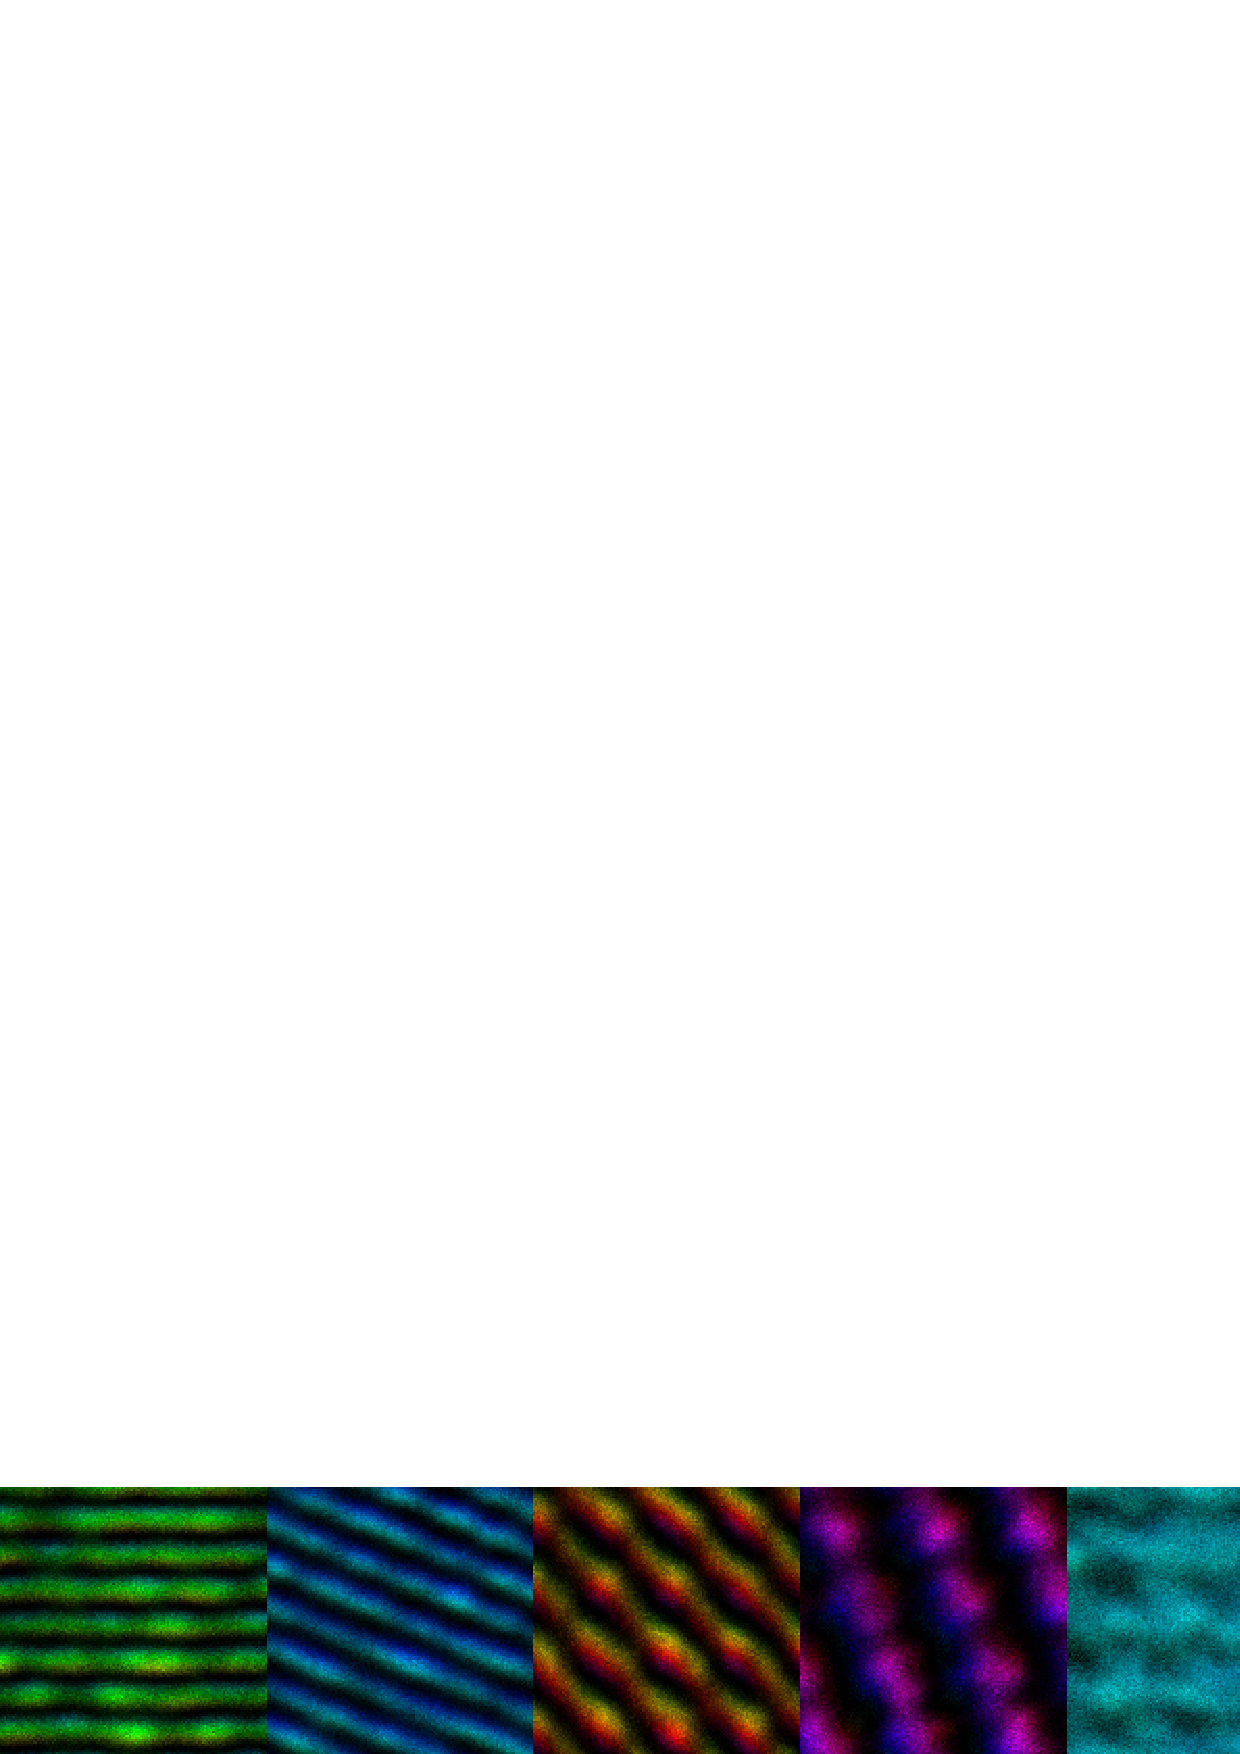
\includegraphics{tmp/out.pdf}
%\caption{How do the font sizes look?}
%\end{figure}

\bibliographystyle{plain}
\bibliography{bibliography}

\appendix

\chapter{Protocols}
\section{Sputtering}
\section{Functionalizing Nanoparticles}
\section{Microfluidics}
\section{Sping Coating of Cytop}

\chapter{Reference Data}
Several datasets were produced during the course of this dissertation which
might be useful to the reader.  They are presented here.
\section{Physical Properties of SPP Propagation}
%\import{dispersion/}{sptable_632.tex}

\section{The Three Layer Fresnel System}
%% you will have to fix the path in the following file
%\import{fresnel_plots/}{allthreelayerfresnel}

\section{Complex Permittivities and Permiabilities of Metals}
%\import{eps_plots/}{allmetals}


\section{Abbreviations}
%\begin{table}
% \begin{tabular}
%  SPP & surface plasmon polariton
%  LRSPP & long range surface plasmon polariton
% \end{tabular}
%\end{table}

\chapter{Miscellaneous}
\section{Colophon}
This document was typeset using pdf\TeX. All
plots were rendered using pgfplots~\cite{feuersangerpgfplots} with styles influenced by
Eduard Tufte~\cite{tufte1983visual}~\cite{tufte1991envisioning}. Colors were chosen
from datasets researched by Jan Brewer~\cite{harrower2003colorbrewer}.
Schematics and other line drawings were prepared using Inkscape. Generation
of text was done under Arch Linux using \texttt{vim}.  Some tables were
pre-processed using LyX.

The Monte Carlo simulations were written in \texttt{c} with pararallelism
accomplished using \texttt{mpi}. The vortex tracking and image processing
algorithms were written in \texttt{octave}.  Weirdospace images were
processed using python and scipy/numpy.  Parallel execution was done at at
the FAU RRZE, Erlangen, Germany.

\end{document}

% MISSING A HOME
% surface roughness parameters
